\documentclass[12pt]{article}
\usepackage[left=1cm, right=1cm, top=2cm,bottom=1.5cm]{geometry} 

\usepackage[parfill]{parskip}
\usepackage[utf8]{inputenc}
\usepackage[T2A]{fontenc}
\usepackage[russian]{babel}
\usepackage{enumitem}
\usepackage[normalem]{ulem}
\usepackage{amsfonts, amsmath, amsthm, amssymb, mathtools}

\usepackage{tabularx}
\usepackage{hhline}

\usepackage{accents}
\usepackage{fancyhdr}
\pagestyle{fancy}
\renewcommand{\headrulewidth}{1.5pt}
\renewcommand{\footrulewidth}{1pt}

\usepackage{graphicx}
\usepackage[figurename=Рис.]{caption}
\usepackage{subcaption}
\usepackage{float}

%%Наименование папки откуда забирать изображения
\graphicspath{ {./images/} }

%%Изменение формата для ввода доказательства
\renewcommand{\proofname}{$\square$  \nopunct}
\renewcommand\qedsymbol{$\blacksquare$}

%%Изменение отступа на таблицах
\addto\captionsrussian{%
	\renewcommand{\proofname}{$\square$ \nopunct}%
}
%% Римские цифры
\newcommand{\RN}[1]{%
	\textup{\uppercase\expandafter{\romannumeral#1}}%
}

%% Для удобства записи
\newcommand{\MR}{\mathbb{R}}
\newcommand{\MC}{\mathbb{C}}
\newcommand{\MQ}{\mathbb{Q}}
\newcommand{\MN}{\mathbb{N}}
\newcommand{\MZ}{\mathbb{Z}}
\newcommand{\MTB}{\mathbb{T}}
\newcommand{\MTI}{\mathbb{I}}
\newcommand{\MI}{\mathrm{I}}
\newcommand{\MJ}{\mathrm{J}}
\newcommand{\MH}{\mathrm{H}}
\newcommand{\MT}{\mathrm{T}}
\newcommand{\MU}{\mathcal{U}}
\newcommand{\MV}{\mathcal{V}}
\newcommand{\MB}{\mathcal{B}}
\newcommand{\MW}{\mathcal{W}}
\newcommand{\ML}{\mathcal{L}}
\newcommand{\VN}{\varnothing}
\newcommand{\VE}{\varepsilon}

\theoremstyle{definition}
\newtheorem{defn}{Опр:}
\newtheorem{rem}{Rm:}
\newtheorem{prop}{Утв.}
\newtheorem{exrc}{Упр.}
\newtheorem{lemma}{Лемма}
\newtheorem{theorem}{Теорема}
\newtheorem{corollary}{Следствие}

\newenvironment{cusdefn}[1]
{\renewcommand\thedefn{#1}\defn}
{\enddefn}

\DeclareRobustCommand{\divby}{%
	\mathrel{\text{\vbox{\baselineskip.65ex\lineskiplimit0pt\hbox{.}\hbox{.}\hbox{.}}}}%
}
%Короткий минус
\DeclareMathSymbol{\SMN}{\mathbin}{AMSa}{"39}
%Длинная шапка
\newcommand{\overbar}[1]{\mkern 1.5mu\overline{\mkern-1.5mu#1\mkern-1.5mu}\mkern 1.5mu}
%Функция знака
\DeclareMathOperator{\sgn}{sgn}

%Функция ранга
\DeclareMathOperator{\rk}{\text{rk}}

%Обозначение константы
\DeclareMathOperator{\const}{\text{const}}

\DeclareMathOperator*{\dsum}{\displaystyle\sum}
\newcommand{\ddsum}[2]{\displaystyle\sum\limits_{#1}^{#2}}

%Интеграл в большом формате
\DeclareMathOperator{\dint}{\displaystyle\int}
\newcommand{\ddint}[2]{\displaystyle\int\limits_{#1}^{#2}}
\newcommand{\ssum}[1]{\displaystyle \sum\limits_{n=1}^{\infty}{#1}_n}

\newcommand{\smallerrel}[1]{\mathrel{\mathpalette\smallerrelaux{#1}}}
\newcommand{\smallerrelaux}[2]{\raisebox{.1ex}{\scalebox{.75}{$#1#2$}}}

\newcommand{\smallin}{\smallerrel{\in}}
\newcommand{\smallnotin}{\smallerrel{\notin}}

\newcommand*{\medcap}{\mathbin{\scalebox{1.25}{\ensuremath{\cap}}}}%
\newcommand*{\medcup}{\mathbin{\scalebox{1.25}{\ensuremath{\cup}}}}%

\makeatletter
\newcommand{\vast}{\bBigg@{3.5}}
\newcommand{\Vast}{\bBigg@{5}}
\makeatother

%Промежуточное значение для sup\inf, поскольку они имеют разную высоту
\newcommand{\newsup}{\mathop{\smash{\mathrm{sup}}}}
\newcommand{\newinf}{\mathop{\mathrm{inf}\vphantom{\mathrm{sup}}}}

%Скалярное произведение
\DeclarePairedDelimiterX{\inner}[2]{\langle}{\rangle}{#1, #2}

%Подпись символов снизу
\newcommand{\ubar}[1]{\underaccent{\bar}{#1}}

%% Шапка для букв сверху
\newcommand{\wte}[1]{\widetilde{#1}}

%%Функция для обозначения равномерной сходимости по множеству
\newcommand{\uconv}[1]{\overset{#1}{\rightrightarrows}}
\newcommand{\uconvm}[2]{\overset{#1}{\underset{#2}{\rightrightarrows}}}


%%Функция для обозначения нижнего и верхнего интегралов
\def\upint{\mathchoice%
	{\mkern13mu\overline{\vphantom{\intop}\mkern7mu}\mkern-20mu}%
	{\mkern7mu\overline{\vphantom{\intop}\mkern7mu}\mkern-14mu}%
	{\mkern7mu\overline{\vphantom{\intop}\mkern7mu}\mkern-14mu}%
	{\mkern7mu\overline{\vphantom{\intop}\mkern7mu}\mkern-14mu}%
	\int}
\def\lowint{\mkern3mu\underline{\vphantom{\intop}\mkern7mu}\mkern-10mu\int}


\begin{document}
\lhead{Математический анализ - \RN{3}}
\chead{Шапошников С.В.}
\rhead{Лекция - 25}
\section*{Свёртка функций: мотивация} 
Для более полного понимания понятия свёртки начнём с физической интерпритации (нестрогой). Представим, что есть некоторое устройство: на вход подается сигнал, на выходе получается сигнал. 
\begin{figure}[H]
	\centering
	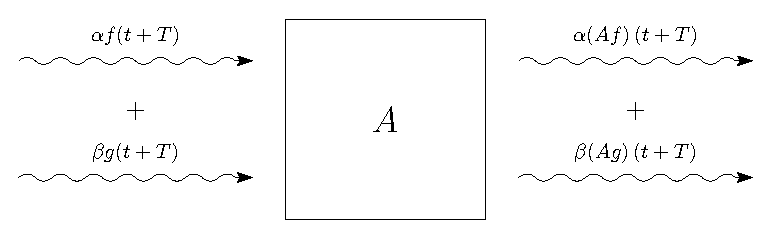
\includegraphics[width=0.65\textwidth]{MA3L25_1.eps}
	\label{MA3L25_1}
	\caption{Физическая мотивация свёртки.}
	\label{fig: свёртка}
\end{figure}
Это устройство обладает двумя свойствами: \uwave{\textbf{линейностью}} и \uwave{\textbf{независимостью от времени}}. Например, весы: сумма двух грузов равна сумме весов, масштабирование работает по весу, как взвешивали вчера, так будут взвешивать и сегодня. Или, например, радиоприемник: суперпозиция сигналов будет выдаваться суперпозицией сигналов, работа вчера не будет отличаться от работы сегодня.

Формализуя, под прибором будем понимать некоторый оператор $A$ на функциях:
$$
	A \colon \mathcal{F} \to \mathcal {F}, \, \mathcal{F} =\{\text{Пространство функций на } \MR\}
$$
Под входящим сигналом будем понимать функцию $f(t)$ на $\MR$, а под выходящим сигналом будем понимать функцию $Af$, также на $\MR$. Тогда свойства прибора будут формализованы так:
\begin{enumerate}[label=(\arabic*)]
	\item \uwave{\textbf{Линейность}}: $A(\alpha f(t) + \beta g(t)) =\alpha Af(t) + \beta Ag(t)$;
	\item \uwave{\textbf{Независимость от времени}}: $\forall \tau \in \MR, \, T_\tau f(t) = f(t - \tau), \, A(T_\tau f(t)) = T_\tau (Af(t))$;
\end{enumerate}
\begin{rem}
	Последнее математически обозначает, что оператор $A$ коммутирует с оператором сдвига $T_\tau$.
\end{rem}
Типичный пример для такой ситуации - закон движения, описывающийся законами Ньютона. Многие колебательные, волновые движения могут иметь следующую форму:
$$
	\left\{
	\begin{array}{lcc}
		\ddot{x} + a\dot{x} + bx &=& f(x)\\
		x(0) = \dot{x}(0) &=& 0
	\end{array}
	\right.	
$$
В начальный момент времени всё находилось в состоянии покоя: у материальной точки не было скорости, стартовая координата была в нуле, затем стали действовать на эту точку силой $f(t)$ и она стала двигаться, при этом её держит какая-то пружина ($bx$) и есть трение ($a \dot{x}$). 

Таким образом, прибор устроен так: подаете на вход силу $f(t)$, а на выходе получаете описание траектории во времени $x(t)$ - функция того, как будет двигаться материальная точка. Проверим, что интересующее сопоставление: $f(t) \to x(t)$ обладает свойствами оператора выше:
\begin{enumerate}[label=(\arabic*)]
	\item Поскольку уравнение линейное, то если $f(t)$ распалось в сумму, то и решение будет строиться как сумма. Если $f(t)$ умножить на константу, то и решение $x(t)$ надо умножить на константу $\Rightarrow$ сопоставление: $f(t) \to x(t)$ обладает свойством линейности;
	
	\item Так как слева в первом уравнении ничего не зависит от $t$, то сдвинуть $f(t)$ будет всё равно что сдвинуть $x(t) \Rightarrow$ если хотим найти закон движения со сдвигом, то можно просто сдвинуть $f(t)$ и посмотреть что получится;
\end{enumerate}
Многие физические законы описываются как некий черный ящик на который вы подаете функцию и из которого получаете функцию в ответ. Замечательно, что это очень общая схема лишь с двумя свойствами, без конкретизации того, как именно работает этот черный ящик.

Возникает вопрос, как описать действия такого прибора? Можно ли ввести какие-то эталонные функции, посмотреть как ведет себя прибор на них и дальше уже описать его действия, не используя сам прибор. Оказывается можно и это будут так называемые точечные импульсы.

\begin{figure}[H]
	\centering
	\includegraphics[width=0.3\textwidth]{MA3L25_2.eps}
	\label{MA3L25_2}
	\caption{Точечные импульсы.}
	\label{fig: Функции точечных импульсов}
\end{figure}

\begin{defn}
	Последовательность функций: 
	$$
		\psi_N(x) = \left\{
		\begin{array}{ll}
			N,& x \in \left[0,\frac{1}{N}\right]\\[4pt]
			0, & x \in \MR \setminus \left[0,\frac{1}{N}\right]
		\end{array}
		\right., \, \forall N \in \MN 
	$$ 
	называется \uwave{функциями точечных импульсов}.
\end{defn}
Отметим, что интегралы от этих функций всё время равны $1$. Представим, что мы взяли наш прибор и померили выходной сигнал на каждой такой функции и посмотрели, что будет на $N \to \infty$. Эвристически предположим, что есть сходимость к некоторой $E(x)$:
$$
	A \psi_N(x) \xrightarrow[N \to \infty]{} E(x)
$$
\begin{defn}
	Функция $E(x) = \lim\limits_{N \to \infty}A \psi_N(x)$ называется \uwave{аппаратной функцией}.
\end{defn}
Оказывается, что всё действие прибора описывается этой функцией и с помощью неё можно описать работу прибора на любом входном сигнале. Рассмотрим непрерывные функции с компактным носителем, то есть: $f \in C(\MR)$ и $f \equiv 0$ вне некоторого отрезка $[-c,c]$.
\begin{figure}[H]
	\centering
	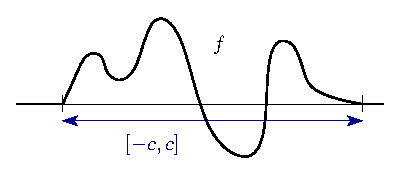
\includegraphics[width=0.4\textwidth]{MA3L25_3.eps}
	\label{MA3L25_3}
	\caption{Функция с компактным носителем.}
	\label{fig: Функция с компактным носителем}
\end{figure}
В таком случае мы можем представить такие функции в виде следующей суммы:
$$
	f(x) \approx \ddsum{k \in \MZ}{}\dfrac{1}{N}{\cdot}f\left(\tfrac{k}{N}\right){\cdot}\psi_N\left(x - \tfrac{k}{N}\right)
$$
Графиком приближения $f$ будут ступенчатые функции по всей $\MR$ (чем-то похоже на конструкции при построении интеграла Римана).
\begin{figure}[H]
	\centering
	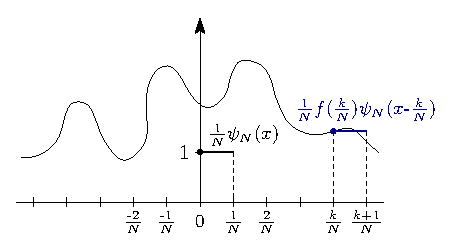
\includegraphics[width=0.5\textwidth]{MA3L25_4.eps}
	\label{MA3L25_4}
	\caption{Приближение функции $f(x)$.}
	\label{fig: Приближение функции $f(x)$}
\end{figure}
Поскольку вне некоторого отрезка $f$ равна нулю, на отрезке равномерно непрерывна, то приближение тоже будет равномерным. Естественно считать, что в приборе (операторе $A$) есть некоторые свойства непрерывности и если мы равномерно приближаемся, то можно менять местами $A$ и предел, тогда:
$$
	Af(x) = A\left(\lim\limits_{N\to \infty}\ddsum{k \in \MZ}{}\dfrac{1}{N}{\cdot}f\left(\tfrac{k}{N}\right){\cdot}\psi_N\left(x - \tfrac{k}{N}\right) \right) = \lim\limits_{N \to \infty}A\left(\ddsum{k \in \MZ}{}\dfrac{1}{N}{\cdot}f\left(\tfrac{k}{N}\right){\cdot}\psi_N\left(x - \tfrac{k}{N}\right)\right) = 
$$
$$
	= \lim\limits_{N \to \infty}\ddsum{k \in \MZ}{}\dfrac{1}{N}{\cdot}f\left(\tfrac{k}{N}\right){\cdot}(A\psi_N)\, \left(x -\tfrac{k}{N}\right) = \lim\limits_{N \to \infty}\ddsum{k \in \MZ}{}\dfrac{1}{N}{\cdot}f\left(\tfrac{k}{N}\right){\cdot}E\left(x -\tfrac{k}{N}\right) = \ddint{-\infty}{+\infty}f(t)E(x - t)dt
$$
где в последней строчке, во втором равенстве мы эвристически перешли к аппаратной функции и получили Риманову сумму. Таким образом, мы получили:
$$
	Af(x) = \ddint{-\infty}{+\infty}f(t)E(x - t)dt
$$
И пользовались всего тремя свойствами: линейностью, перестановочностью со сдвигами и пользовались какого-то сорта непрерывностью, чтобы менять местами разные пределы. Эту непрерывность несложно обосновать строго, например, для перестановочности $A$ и равномерного предела функций $f_N(x)$:
$$
	f_N(x) \uconv{} f, \, f_N(x) \equiv 0, \, \forall x \in \MR \setminus [-c,c] \Rightarrow \forall x \in \MR, \, Af_N(x) \to Af(x)
$$  
Можно и дальше делать строгие обоснование, только в рамках данного курса мы это делать не будем. В книге Хёрмандера (оценки для операторов) есть некоторые детали про свёртку (теорема Шварца).

\newpage
\section*{Свёртка функций}
\begin{defn}
	Выражение $\ddint{-\infty}{+\infty}f(t)g(x - t)dt$ называется \uwave{свёрткой функций} $f$ и $g$ и обозначается $f*g(x)$.
\end{defn}
Возникают вопросы: когда это выражение имеет смысл, когда этот интеграл определен? Интеграл несобственный, две особенности $\Rightarrow$ имеет смысл разбить на два и оба интеграла должны сходиться.

Пусть $f(x)$ и $g(x)$ интегрируемы по Риману на всяком отрезке $[a,b] \subset \MR \Rightarrow f(t)g(x-t)$ - интегрируема на $[a,b], \, \forall [a,b]\subset \MR$.
Далее везде будем предполагать, что это так.
 
\begin{prop}
	Для существования свёртки $f*g(x), \, \forall x \in \MR$ достаточно хотя бы одного из следующих условий:
	\begin{enumerate}[label=(\arabic*)]
		\item $\ddint{-\infty}{+\infty}|f(t)|dt$ -  сходится и $g(t)$ - ограничена;
		\item $f(x)$ или $g(x)$ \uwave{финитна}, то есть равна нулю вне некоторого отрезка;
		\item $\ddint{-\infty}{+\infty}|f(t)|^2dt$ и $\ddint{-\infty}{+\infty}|g(t)|^2dt$ - сходятся;
	\end{enumerate}
\end{prop}
\begin{rem}
	Заметим, что все эти три условия не одинаковы. 
	\begin{enumerate}[label=(\arabic*)]
		\item Не требуется зануления хотя бы одной из функций вне некоторого отрезка;
		\item Если одна из функций зануляется, то нет никакого несобственного интеграла, поскольку в этом случае интеграл будет браться по некоторому отрезку $\Rightarrow$ мы работаем с конечным интегралом;
		\item Не требуется интегрируемости $f(x)$ и $g(x)$, а требуется интегрируемость квадратов и возможно следующее:
		$$
			\ddint{-\infty}{+\infty}\dfrac{1}{1 + |t|}dt \not< \infty, \, \ddint{-\infty}{+\infty}\dfrac{1}{(1 + |t|)^2}dt < \infty
		$$
	\end{enumerate}
\end{rem}
\begin{rem}
	Также заметим, что это не все возможные случаи существования свёртки и это не самые общие условия, когда она существует. В других курсах, далее, свойства свёртки будут ещё раз изучаться.
\end{rem}
\begin{proof}
	По определению:
	$$
		f*g(x) = \ddint{-\infty}{+\infty}f(t)g(x-t)dt
	$$
	\begin{enumerate}[label=(\arabic*)]
		\item Очевидно, по признаку Вейерштрасса $\Rightarrow$ сразу будет сходимость;
		\item Если какая-то функция финитна, то $f(t)g(x - t) = 0$ вне какого-то отрезка $\Rightarrow$ интеграл собственный $\Rightarrow$ существует по интегрируемости функций по Риману;
		\item Из неравенства средних:
		$$
			|f(t)g(x - t)| \leq \dfrac{1}{2}|f(t)|^2 + \dfrac{1}{2}|g(x - t)|^2
		$$ 
		Рассмотрим интегралы:
		$$
			\ddint{-\infty}{+\infty}|f(t)|^2dt < \infty, \, \ddint{-\infty}{+\infty}|g(x - t)|^2dt = \ddint{-\infty}{+\infty}|g(s)|^2ds < \infty \Rightarrow \ddint{-\infty}{+\infty}|f(t)g(x - t)|dt < \infty
		$$
		Следовательно, по признаку Вейерштрасса будет сходимость;
	\end{enumerate}
\end{proof}
\section*{Свойства свёртки функций}

\begin{prop}
	Пусть $f*g(x)$ существует $\forall x \in \MR$, тогда:
	\begin{enumerate}[label=(\arabic*)]
		\item Существует $g*f(x), \, \forall x \in \MR$ и $g*f(x) =f*g(x)$;
		\item Если $\exists \, f_1 *g(x), f_2*g(x)$, то $\forall \alpha, \beta, \, \exists \, (\alpha f_1 + \beta f_2)*g(x) = \alpha (f_1 *g)(x) + \beta(f_2*g)(x)$;
		\item Для финитных, непрерывных $f,g,h$ верно: $h*(g*f)(x) = (h*g)*f(x)$;
		\item Оператор сдвига коммутирует со свёрткой: $T_\tau(f*g) (x) = f*(T_\tau g)(x)$; 
	\end{enumerate}
\end{prop}
\begin{rem}
	Получаем свойства похожие на свойства кольца в пространстве функций, где свёртка это операция ``умножения''. Свойство $(1)$ - коммутативность, $(2)$ - дистрибутивность, $(3)$ - ассоциативность, но не хватает единицы в этом пространстве такой, чтобы $f*\mathbf{1} = f$. Если бы была единица, то получилось бы на фунциях придумать умножение в виде свёртки.
\end{rem}
\begin{proof}\hfill
	\begin{enumerate}[label=(\arabic*)]
		\item По свойствам несобственного интеграла, если интеграл до замены есть, то и после неё он сходится. Тогда, по определению:
		$$
			\ddint{-\infty}{+\infty} f(t)g(x -t)dt = |t = x - s| = \ddint{-\infty}{+\infty} f(x - s)g(s)ds = g*f(x) < \infty 
		$$
		\item По условию, существуют следующие интегралы:
		$$
			\ddint{-\infty}{+\infty} f_1(t)g(x -t)dt < \infty, \, \ddint{-\infty}{+\infty} f_2(t)g(x -t)dt < \infty
		$$
		Тогда по определению линейности интеграла будет существовать интеграл от линейной комбинации функций и верно равенство:
		$$
			\ddint{-\infty}{+\infty}\left(\alpha f_1(t) + \beta f_2(t)\right)g(x -t)dt = \alpha \ddint{-\infty}{+\infty} f_1(t)g(x -t)dt + \beta \ddint{-\infty}{+\infty} f_1(t)g(x -t)dt < \infty
		$$
		\setcounter{enumi}{3}
		\item По условию, мы требуем $\exists \, f*g(x), \, \forall x \in \MR$, возьмем сдвиг:
		$$
			T_\tau(f*g)(x) = f*g(x-t) = \ddint{-\infty}{+\infty}f(t){\cdot}g(x - \tau -t)dt = \ddint{-\infty}{+\infty}f(t){\cdot}(T_\tau g)(x - t)dt = f*(T_\tau g)(x)
		$$
		\setcounter{enumi}{2}
		\item Пусть $h,f,g$ - финитны и непрерывны, тогда по определению:
		$$
			h*(f*g)(x) =
			\ddint{-\infty}{+\infty}h(t){\cdot}\!\left(f*g(x-t)\right)dt = 
			\ddint{-\infty}{+\infty}h(t){\cdot}\!\!\left(\,\ddint{-\infty}{+\infty}f(s)g(x-t -s)ds\right)dt
		$$
		все интегралы выше при условиях финитности это собственные интегралы по конечным промежутка от непрерывных функций. Аналогично для правой части равенства:
		$$
			(h*g)*f(x) = \ddint{-\infty}{+\infty}\left( h*f(v)\right){\cdot}g(x-v)dv =  \ddint{-\infty}{+\infty}\left(\, \ddint{-\infty}{+\infty}h(u)f(v -u)du\right){\cdot}g(x-v)dv
		$$
		Внесём под первый интеграл оставшиеся слагаемые и сделаем замену под интегралом:
		$$
			\ddint{-\infty}{+\infty}\left(\,\ddint{-\infty}{+\infty}h(t){\cdot}f(s){\cdot} g(x-t -s)ds\right)dt = |s = v - t| = \ddint{-\infty}{+\infty}\left(\,\ddint{-\infty}{+\infty}h(t){\cdot}f(v-t){\cdot} g(x-v)dv\right)dt
		$$
		Меняем местами интегралы, в силу финитности и непрерывности функций, тогда:
		$$
			\ddint{-\infty}{+\infty}\left(\,\ddint{-\infty}{+\infty}h(t){\cdot}f(v-t){\cdot} g(x-v)dv\right)dt = \ddint{-\infty}{+\infty}\left(\,\ddint{-\infty}{+\infty}h(t){\cdot}f(v-t){\cdot} g(x-v)dt\right)dv = 
		$$
		$$
			=|u = t| = \ddint{-\infty}{+\infty}\left(\,\ddint{-\infty}{+\infty}h(u){\cdot}f(v-u){\cdot} g(x-v)du\right)dv = \ddint{-\infty}{+\infty}\left( h*f(v)\right){\cdot}g(x-v)dv = (h*g)*f(x)
		$$
	\end{enumerate}
\end{proof}

Остается вопрос, а существует ли для свёртки единица? Пусть такая функция существует для финитных и непрерывных функций (обозначим их пространство $\mathcal{G}$), обозначем её как $g$, тогда:
$$
	\forall f \in \mathcal{G}, \, \forall x \in \MR, \, f*g(x) = f(x) \Rightarrow \ddint{-\infty}{+\infty}f(x-t)g(t)dt = f(x)
$$
Если $g(t) \equiv 1$, то слева получим константу по интегралу, а справа функцию $\Rightarrow$ не подходит. Поскольку мы хотим, чтобы равенство выполнялось для всех $x$, то рассмотрим его в нуле:
$$
	x = 0 \Rightarrow \ddint{-\infty}{+\infty}f(-t)g(t)dt = f(0)
$$
Рассмотрим следующую последовательность финитных, непрерывных функций:
$$
	\forall n \in \MN, \, f_n(x) = 
	\left\{
		\begin{array}{rl}
			0, & x \in \MR \setminus \left[-\frac{1}{n},\frac{1}{n}\right] \\[10pt]
			1 + \dfrac{x}{n}, & x \in  \left[-\frac{1}{n}, 0\right]\\[10pt]
			1 - \dfrac{x}{n}, & x \in \left[0, \frac{1}{n}\right]
		\end{array}
	\right.
$$
\begin{figure}[H]
	\centering
	\includegraphics[width=0.5\textwidth]{MA3L25_5.eps}
	\label{MA3L25_5}
	\caption{Последовательность треугольников $f_n(x)$.}
	\label{fig: Последовательность треугольников}
\end{figure}
Они представляют из себя треугольники на отрезке $\left[-\frac{1}{n},\frac{1}{n}\right]$ с вершиной в точке $0$ и ноль вне этого отрезка, где $f(0) = 1$. Попробуем для такой последовательности функций вычислить значение свёртки в точке $0$, учитывая интегрируемость функции $g(x)$, а следовательно её ограниченность:
$$
	1 = f_n (0) = \ddint{-\frac{1}{n}}{\frac{1}{n}}f_n(-t)g(t)dt \leq \ddint{-\frac{1}{n}}{\frac{1}{n}}1{\cdot}C dt = \dfrac{2C}{n} \xrightarrow[n \to \infty]{}0
$$
В результате, получили противоречие. Справиться можно было бы с этим увеличивая функцию $g(t)$, то есть она должна была бы компенсировать сжимание области интегрирования. Как итого, среди функций единицы нет, но это не означает, что её вообще нет. Единица есть в так называемых обобщенных функциях (будет изучаться на $3$-ьем курсе). 
\begin{rem}
	С чем-то похожим мы сталкиваемся при изучении вещественных и рациональных чисел, вещественных чисел изначально нет среди рациональных, нет никакого рационального числа, которое могло быть равно $\sqrt{2}$. Вещественные числа мы получаем предельным переходом, как пределы последовательностей рациональных чисел. По аналогии в этой ситуации, нам не хватает функций.
\end{rem}

\subsection*{Дельтаобразные последовательности}
Найдем эту единицу для свёртки среди последовательностей функций.

\begin{defn}
	\uwave{Дельтаобразной последовательностью} функций называется всякая последовательность функций $\{\omega_n\}$, удовлетворяющая свойствам:
	\begin{enumerate}[label=\arabic*)]
		\item $\omega_n$ - интегрируема и $\ddint{-\infty}{+\infty}\omega_n(t)dt = 1$;
		\item $\omega_n \geq 0$;
		\item $\forall \delta > 0, \, \ddint{|t|\geq \delta}{}\omega_n(t)dt \xrightarrow[n \to \infty]{} 0$;
	\end{enumerate}
\end{defn}

Чтобы понять устройство этих функций, рассмотрим крайне показательный пример.

\textbf{Пример}: Пусть $\psi \geq 0, \, \ddint{-\infty}{+\infty}\psi(x)dx = 1, \, \forall n \in \MN, \, \omega_n(x) = n\psi(nx)$, тогда $\{\omega_n\}$ - это дельтаобразная последовательность:
\begin{enumerate}[label=\arabic*)]
	\setcounter{enumi}{1}
	\item Просто по определению: $\omega_n(x) = n\psi(nx) \geq 0$;
	\setcounter{enumi}{0}
	\item $\ddint{-\infty}{+\infty}\omega_n(t)dt = \ddint{-\infty}{+\infty}n\psi(nt)dt = |nt = s| = \ddint{-\infty}{+\infty}\psi(s)ds = 1$;
	\setcounter{enumi}{2}
	\item $\forall \delta > 0, \, \ddint{|t|\geq \delta}{}\omega_n(t)dt = \ddint{|t|\geq \delta}{}n\psi(nt)dt =|nt =s| = \ddint{-\infty}{-n\delta}\psi(s)ds + \ddint{n\delta}{+\infty}\psi(s)ds \xrightarrow[n \to \infty]{} 0$, поскольку это хвосты сходящегося несобственного интеграла;
\end{enumerate}
\begin{figure}[H]
	\centering
	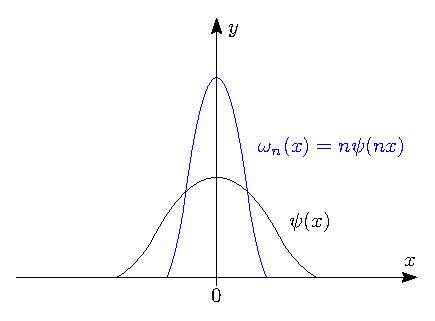
\includegraphics[width=0.4\textwidth]{MA3L25_6.eps}
	\label{MA3L25_6}
	\caption{Последовательность $\delta$-образных функций $\omega_n(x)$.}
	\label{fig: Последовательность дельтаобразных.}
\end{figure}
Видно, что последовательность $\omega_n(x)$ поджимаются к нулю по $x$ и вытягиваются по $y$. И происходит то, чего нам не хватало при доказательстве отсутствия единицы для свёртки.

\begin{rem}
	Заметим также, что функции точечных импульсов, которые мы разбирали в мотивации свёртки, построены из функции-индикатора на $[0,1]$:
	$$
		\psi(x) = \MTI_{[0,1]}(x) \Rightarrow
		\psi_N(x) = \left\{
		\begin{array}{ll}
			N,& x \in \left[0,\frac{1}{N}\right]\\[4pt]
			0, & x \in \MR \setminus \left[0,\frac{1}{N}\right]
		\end{array}
		\right. = N\psi(Nx), \, \forall N \in \MN 
	$$ 	
\end{rem}
Дельтаобразная последовательность названа так в честь физика Дирака, который указал, что для многих физических моделей полезно рассматривать функцию Дирака.
\begin{defn}
	\uwave{Функцией Дирака} будем называть следующий объект:
	$$
		\delta(x) = \left\{
		\begin{array}{rl}
			0, & x \neq 0\\
			\infty, & x =0
		\end{array}
		\right., \, \ddint{-\infty}{+\infty}\delta(x)dx = 1
	$$
\end{defn}
Формально, в математике нет такой функции (среди функций), но математики придумали как такую функцию можно прописать. Один из способов это через обобщенные функции, который мы не будем здесь рассматривать, а другой способ - заменить её дельтаобразной последовательностью: $\omega_n(x) \to \delta (x)$. Естественно хотелось бы понять, нашли ли мы искомую единицу для свёртки?

\begin{theorem}
	Пусть $f$ - непрерывная и ограниченная, $\{\omega_n\}$ - это дельтаобразная последовательность. Тогда: $f *\omega_n(x) \uconvm{}{n \to \infty}f(x)$ на всяком отрезке $[a,b] \subset \MR$.
\end{theorem} 

\end{document}